% \addtocontents{toc}{\protect\newpage}
\section{Empirical Study}\label{sec:empirical-study}

In this section, we demonstrate the efficacy of machine learning for trade classification in an empirical setting. We begin by outlining the dataset construction.

\subsection{Data and Data Preparation}\label{sec:data-and-data-preparation}

The following chapter describes the construction of datasets, that suffice the data requirements of classical trade classification rules and for our machine learning models. We also discuss how we define and infer the true trade initiator.

\subsubsection{Data Collection}\label{sec:data-collection}


Testing the empirical accuracy of our approaches requires option trades where the true initiator is known. To arrive at a labeled sample, we combine data from four individual data sources. Our primary source is LiveVol, which records option trades executed at US option exchanges at a transaction level. We limit our focus to option trades executed at the \gls{CBOE} and \gls{ISE}. LiveVol contains both trade and matching quote data. Like most proprietary data sources, it does not distinguish the initiator nor does it include the involved trader types. For the \gls{CBOE} and \gls{ISE} exchange, the \gls{ISE} Open/Close Trade Profile and \gls{CBOE} Open-Close Volume Summary contain the buy and sell volumes for the option series by trader type aggregated on a daily level. A combination of the LiveVol dataset with the open/close data, allows us to infer the trade initiator for a subset of trades. For evaluation and use in some of our machine learning models, we acquire additional underlying and option characteristics from IvyDB's OptionMetrics.

In \cref{sec:trade-initiator} we discussed three views on the trade initiator. Due to the absence of order entry times or order types in our data sources, we define the trade initiator based on the position relative to the market maker, who caters to the liquidity demand. Specifically, we classify customer trades as buyer-initiated if the trade is due to a customer buy order and as seller-initiated for customer sales. As previous literature, e.g., \textcite[][4276]{garleanuDemandBasedOptionPricing2009} suggests that trader types, for example, proprietary traders, have a similar role to market makers by supplying liquidity, we limit our analysis to trades between customers and market makers for which the picture is unambiguous. Our definition is consistent with \textcite[][8]{grauerOptionTradeClassification2022}.


Our sample construction follows \textcite[][7--9]{grauerOptionTradeClassification2022}, fostering comparability between both works. Our analysis is conducted on transactions at the \gls{ISE} and \gls{CBOE}. We acquire transaction-level options trade data for all major US exchanges from LiveVol. The dataset is tabular and each record is time-stamped to the second. For each transaction, the executing exchange, trade price, trade volume, quotes, and quote sizes for the exchanges where the option is quoted, as well as the \gls{NBBO} are recorded. This is sufficient to estimate the quote rule, depth rule, and trade size rule. In addition, for tick-based algorithms, we add the previous and subsequent distinguishable trade prices. We can uniquely identify the traded option series from a distinct key consisting of the underlying, expiration date, option type, and strike price. To purge the data of potential errors, we filter out:
\begin{enumerate}[label=(\roman*),noitemsep]
    \item trades with a trade price $\leq \SI{0}[\$]{}$,
    \item trades with a trade volume $\leq 0$ or $\ge \num{10000000}$ contracts,
    \item canceled or duplicated trades,
    \item entries with multiple underlying symbols for the same root.
\end{enumerate}


The open/close datasets for the \gls{ISE} and \gls{CBOE} contain the daily buy and sell volumes for the option series by trader type, the trade volume, and whether a position was closed or opened. Four trader types are available: customer, professional customer, broker/dealer, and firm proprietary. Customer orders are placed by a retail trader or a member of the exchange on behalf of the customer. Professional customers are distinguished from the former by a high trading activity ($\geq390$ orders per day over one month period). Likewise, trades by a member are classified as proprietary, if executed for their account or broker/dealer if placed for non-members of the exchange \autocite[][2]{nasdaqincFrequentlyAskedQuestions2017}. Trades of customers and professional customers are detailed by trade volume ($\leq 100$; 101--199; $> 199$ contracts). As well as, if a position is newly opened or closed. We first sum buy and sell orders of all trader types and volumes to obtain the daily trading volumes at the \gls{ISE} or \gls{CBOE} per option series and day. Separately for the customer buy and sell volumes, we calculate the daily aggregates identified by the account type customer.

To infer the true label, we exploit that, if there were only customer buy or sell orders, hence the customer buy or sell volume equals the daily trading volume, we can confidently sign all transactions for the option series at the specific date and exchange as either buyer- or seller-initiated. Our labeling approach fails in the presence of non-customer or simultaneous customer buy or sell trades. The so-obtained trade initiator is merged with the LiveVol trades of the exchange based on the unique key for the option series.

For the \gls{ISE} trades, our matched sample spans from 2 May 2005 to 31 May 2017 and includes \num{49203747} trades. The period covers the full history of \gls{ISE} open/close data up to the last date the dataset was available to us. Our matched \gls{CBOE} sample consists of \num{37155412} trades between 1 January 2011 and 31 October 2017. The sample period is governed by a paradigm shift in the construction of the \gls{CBOE} open/close dataset and the most recent trade in our LiveVol subscription.

Following our initial rationale to explore semi-supervised methods, we reserve unlabeled trades between 24 October 2012 and 24 October 2013 at the \gls{ISE} for pre- and self-training. We provide further details in \cref{sec:train-test-split}. Since LiveVol doesn't distinguish by trader types, this dataset includes both customer and non-customer trades, as well as simultaneous buy and sell trades on the same day. Within this period, we filter out trades for which the true label can be inferred to avoid overlap with the supervised dataset. This is crucial for self-training, where labeled and unlabeled data are presented to the model simultaneously.

While our procedure makes the inference of the true trade initiator partly feasible, concerns regarding a selection bias due to the excessive filtering have to be raised. We address these concerns and report summary statistics for unmerged and merged sub-samples in \cref{app:summary-statistics}. In the following chapter, we motivate feature engineering, present our feature sets and discuss strategies for transforming features into a form that accelerates the training of our models.

\subsubsection{Data Preprocessing}\label{sec:data-preprocessing}

Classical algorithms infer the initiator of the trade from the \emph{raw} price and quote data. We employ feature engineering to pre-process input data and enhance the convergence and performance of our machine-learning models. Gradient-boosted trees and neural networks, though, flexible estimators have limitations in synthesizing new features from existing ones, as demonstrated in empirical work on synthetic data by \textcite[][4--6]{heatonEmpiricalAnalysisFeature2016}. Specifically, ratios, standard deviations, and differences can be difficult for these models to learn and must therefore be engineered beforehand.

\textbf{Features and Feature Sets}

To establish a common ground, we define three feature sets, abbreviated as \glsdisp{FS}{FS}. These sets are motivated by features inherent to classical heuristics and are consequently derived from quote and price data. Except for a third feature set, which includes option characteristics. Using separate feature sets enhances result transferability.

\begin{ThreePartTable}
    \centering
    \begin{TableNotes}\footnotesize
        \item[*] Notation assumes, that the previous or next trade price is distinguishable. See discussion in \cref{sec:tick-test}.
    \end{TableNotes}
    \begin{longtable}{@{}lllllll@{}}
        \caption[Features and Feature Sets]{Features and feature sets. We divide data into three feature sets: classic, size, and option, aligned with the data requirements of traditional trade classification rules. Feature definitions are derived from rules without quantization, whereby the column source documents the origin. Additional option-specific features are defined in the text.}\label{tab:feature-sets} \\
        \toprule
        Feature Name            & Definition                                                                                                                      & Source               & \gls{FS} Classic                  & \gls{FS} Size                     & \gls{FS} Option                                                                                                                                    \\ \midrule
        \endfirsthead

        \multicolumn{6}{l}{\emph{Continued \tablename~\thetable}}                                                                                                                                                                                                                                                                                                                                                   \\
        \toprule
        Feature Name            & Definition                                                                                                                      & Source               & \gls{FS} Classic                  & \gls{FS} Size                     & \gls{FS} Option                                                                                                                                    \\ \midrule
        \endhead

        \bottomrule
        \endfoot

        \insertTableNotes
        \endlastfoot

        trade price             & $P_{i, t}$                                                                                                                      & tick rule            & \textcolor{viz-green}{\checkmark} & \textcolor{viz-green}{\checkmark} & \textcolor{viz-green}{\checkmark}                                                                                                                  \\
        price lag (ex)          & $P_{i, t-1}^{\mathrm{ex}}$\tnote{*}                                                                                               & tick rule            & \textcolor{viz-green}{\checkmark} & \textcolor{viz-green}{\checkmark} & \textcolor{viz-green}{\checkmark}                                                                                                                  \\
        price lag (all)         & $P_{i, t-1}^{\mathrm{all}}$\tnote{*}                                                                                              & tick rule            & \textcolor{viz-green}{\checkmark} & \textcolor{viz-green}{\checkmark} & \textcolor{viz-green}{\checkmark}                                                                                                                  \\
        price change lag (ex)   & $P_{i, t-1}^{\mathrm{ex}}/P_{i, t}^{\mathrm{ex}}$\tnote{*}                                                                          & tick rule            & \textcolor{viz-green}{\checkmark} & \textcolor{viz-green}{\checkmark} & \textcolor{viz-green}{\checkmark}                                                                                                                  \\
        price change lag (all)  & $P_{i, t-1}^{\mathrm{all}}/P_{i, t}^{\mathrm{all}}$\tnote{*}                                                                        & tick rule            & \textcolor{viz-green}{\checkmark} & \textcolor{viz-green}{\checkmark} & \textcolor{viz-green}{\checkmark}                                                                                                                  \\
        priced lead (ex)        & $P_{i, t+1}^{\mathrm{ex}}$\tnote{*}                                                                                               & rev. tick rule       & \textcolor{viz-green}{\checkmark} & \textcolor{viz-green}{\checkmark} & \textcolor{viz-green}{\checkmark}                                                                                                                  \\
        price lead (all)        & $P_{i, t+1}^{\mathrm{all}}$\tnote{*}                                                                                              & rev. tick rule       & \textcolor{viz-green}{\checkmark} & \textcolor{viz-green}{\checkmark} & \textcolor{viz-green}{\checkmark}                                                                                                                  \\
        price change lead (ex)  & $P_{i, t}^{\mathrm{ex}}/P_{i, t+1}^{\mathrm{ex}}$\tnote{*}                                                                          & rev. tick rule       & \textcolor{viz-green}{\checkmark} & \textcolor{viz-green}{\checkmark} & \textcolor{viz-green}{\checkmark}                                                                                                                  \\
        price change lead (all) & $P_{i, t}^{\mathrm{all}}/P_{i, t+1}^{\mathrm{all}}$\tnote{*}                                                                        & rev. tick rule       & \textcolor{viz-green}{\checkmark} & \textcolor{viz-green}{\checkmark} & \textcolor{viz-green}{\checkmark}                                                                                                                  \\
        bid (all)               & $B_{i, t}^{\mathrm{all}}$                                                                                                         & quote rule           & \textcolor{viz-green}{\checkmark} & \textcolor{viz-green}{\checkmark} & \textcolor{viz-green}{\checkmark}                                                                                                                  \\
        bid (ex)                & $B_{i, t}^{\mathrm{ex}}$                                                                                                          & quote rule           & \textcolor{viz-green}{\checkmark} & \textcolor{viz-green}{\checkmark} & \textcolor{viz-green}{\checkmark}                                                                                                                  \\
        ask (all)               & $A_{i, t}^{\mathrm{all}}$                                                                                                         & quote rule           & \textcolor{viz-green}{\checkmark} & \textcolor{viz-green}{\checkmark} & \textcolor{viz-green}{\checkmark}                                                                                                                  \\
        ask (ex)                & $A_{i, t}^{\mathrm{all}}$                                                                                                         & quote rule           & \textcolor{viz-green}{\checkmark} & \textcolor{viz-green}{\checkmark} & \textcolor{viz-green}{\checkmark}                                                                                                                  \\
        prox. to quotes (ex)    & $\tfrac{2 \left(P_{i, t}^{\mathrm{ex}}- M_{i, t}^{\mathrm{ex}}\right)}{\left(A_{i, t}^{\mathrm{ex}}-B_{i, t}^{\mathrm{ex}}\right)}$     & \gls{EMO}/\gls{CLNV} & \textcolor{viz-green}{\checkmark} & \textcolor{viz-green}{\checkmark} & \textcolor{viz-green}{\checkmark}                                                                                                                  \\
        prox. to quotes (all)   & $\tfrac{2 \left(P_{i, t}^{\mathrm{all}}- M_{i, t}^{\mathrm{all}}\right)}{\left(A_{i, t}^{\mathrm{all}}-B_{i, t}^{\mathrm{all}}\right)}$ & \gls{EMO}/\gls{CLNV} & \textcolor{viz-green}{\checkmark} & \textcolor{viz-green}{\checkmark} & \textcolor{viz-green}{\checkmark}                                                                                                                  \\
        bid ask size ratio (ex) & $\tilde{B}_{i, t}^{\mathrm{ex}}/\tilde{A}_{i, t}^{\mathrm{ex}}$                                                                     & depth rule           &                                   & \textcolor{viz-green}{\checkmark} & \textcolor{viz-green}{\checkmark}                                                                                                                  \\
        bid size (ex)           & $\tilde{B}_{i, t}^{\mathrm{ex}}$                                                                                                  & depth rule           &                                   & \textcolor{viz-green}{\checkmark} & \textcolor{viz-green}{\checkmark}                                                                                                                  \\
        ask size (ex)           & $\tilde{A}_{i, t}^{\mathrm{ex}}$                                                                                                  & depth rule           &                                   & \textcolor{viz-green}{\checkmark} & \textcolor{viz-green}{\checkmark}                                                                                                                  \\
        rel. bid size (ex)      & $\tilde{B}_{i, t}^{\mathrm{ex}}/\tilde{P}_{i, t}^{\mathrm{ex}}$                                                                     & trade size rule      &                                   & \textcolor{viz-green}{\checkmark} & \textcolor{viz-green}{\checkmark}                                                                                                                  \\
        rel. ask size (ex)      & $\tilde{A}_{i, t}^{\mathrm{ex}}/\tilde{P}_{i, t}^{\mathrm{ex}}$                                                                     & trade size rule      &                                   & \textcolor{viz-green}{\checkmark} & \textcolor{viz-green}{\checkmark}                                                                                                                  \\
        trade size              & $\tilde{P}_{i, t}$                                                                                                              & trade size rule      &                                   & \textcolor{viz-green}{\checkmark} & \textcolor{viz-green}{\checkmark}                                                                                                                  \\
        root                    & $\left\{\mathtt{SPY},\ldots\right\}$                                                                                            & option               &                                   &                                   & \textcolor{viz-green}{\checkmark}                                                                                                                  \\
        strike price            & $K_{i}$                                                                                                                       & option               &                                   &                                   & \textcolor{viz-green}{\checkmark}                                                                                                                  \\
        time to maturity        & $\tau_{i,t}$                                                                                                                    & option               &                                   &                                   & \textcolor{viz-green}{\checkmark}                                                                                                                  \\
        moneyness               & $\tfrac{S_{i,t}}{K_{i}}$ or $\tfrac{K_{i}}{S_{i,t}}$                                                                        & option               &                                   &                                   & \textcolor{viz-green}{\checkmark}                                                                                                                  \\
        option type             & $\left\{\mathtt{C},\mathtt{P}\right\}$                                                                                          & option               &                                   &                                   & \textcolor{viz-green}{\checkmark}                                                                                                                  \\
        security type           & $\left\{\mathtt{0},\mathtt{A},\ldots\right\}$                                                                                   & option               &                                   &                                   & \textcolor{viz-green}{\checkmark}                                                                                                                  \\
        volume option series    &                                                                                                                                 & option               &                                   &                                   & \textcolor{viz-green}{\checkmark}                                                                                                                  \\ \bottomrule
    \end{longtable}
\end{ThreePartTable}


Features and feature sets are documented in \cref{tab:feature-sets}.
We aid the models by estimating the change in trade price between the previous and successive distinguishable trades. This is identical to the criterion in the (reverse) tick rule, but in a non-quantized fashion to enforce a richer decision boundary and to surpass hard cut-off points. Similarly, the proximity of the trade price to the quotes, which is the decisive criterion in the quote rule and hybrids thereof is added. The feature value ranges from $\left(-\infty,\infty\right)$ and is $-1$ for trades at the bid, 0 for trades at the mid, and 1 for trades at the ask. Quotes and trade prices are also incorporated as-is.

Our second feature set, named \gls{FS} size, extends the first feature set by the trade size and quoted sizes, required to estimate hybrid rules involving the depth rule and trade size rule. Both rules achieve state-of-the-art performance on option trades when paired with hybrid algorithms and are thus a viable source of features. We model the depth rule as the ratio between ask and bid sizes and the trade size rule as the ratio between the size of the trade and the quoted bid and ask sizes. Since features are not discretized, we obtain a generic formulation of the trade size rule, where part of the quoted size can remain unfilled. This potentially helps to distinguish limit orders from market orders. The trade price and midspread required for the depth rule are already encompassed in the first feature set. More generically, trade size is known to strongly affect classification. For instance, \textcites[][889]{savickasInferringDirectionOption2003}[][537]{ellisAccuracyTradeClassification2000} report that better classification is associated with smaller trades, as smaller trades are more likely to be executed at the quotes. By providing the model with the trade and quoted sizes we hope to make these nuances learnable.

Our largest feature set, abbreviated with \gls{FS} option, also incorporates option characteristics, including the option type among others. By providing unique identifiers for the option series, we can potentially establish connections between transactions when trade initiators divide a single order into sub-orders or rely on complex trades. Similar reasoning applies to the daily volume of the option series. Option features are also informative individually. Time to maturity $\tau_{i,t}$, estimated in months, indirectly affects classification performance. On \gls{CBOE} data in \textcite[][889]{savickasInferringDirectionOption2003}, trades with longer maturities are smaller, hence more likely to be classified correctly. Moreover, time to maturity can be used as a dummy to identify rollovers \autocite[][700]{muravyevOrderFlowExpected2016}. When investors are short in call or put options, they replace expiring for non-expiring options, which creates selling pressure in the non-expiring option. The feature could make the procedure learnable. Related to the time to maturity is moneyness, estimated as the ratio between the price of the underlying $S_{i,t}$ and the strike price $K_{i}$ for calls and the reciprocal for puts. As moneyness is linked to leverage in the investment, we reason that incentives to initiate a trade might vary between buyers and sellers. The classification of index options poses challenges for traditional approaches relative to other security types \autocites[][22]{grauerOptionTradeClassification2022}[][898-899]{savickasInferringDirectionOption2003}. We equip the models with the security type, as well as the option type and root to extend the learnable context.

Arguably, our models have simultaneous access to the previous and successive trade prices and quotes for both the exchange and the \gls{NBBO}, which is an advantage over base rules. As we benchmark against various, stacked hybrid rules, the data requirements are still comparable. We emphasize this aspect, as it is neglected in previous works (cp. \textcites[][485]{blazejewskiLocalNonParametricModel2005}[][48]{ronenMachineLearningTrade2022}[][398]{rosenthalModelingTradeDirection2012}).

\textbf{Numerical Features}

Pricing or quote data can often not be fully reconstructed, resulting in missing values across all features. Decision trees and ensembles thereof can inherently handle $\mathtt{[NaN]}$ values by discarding missing values in the splitting procedure \autocite[][150--152]{breimanClassificationRegressionTrees2017} or by incorporating missing values into the splitting criterion \autocite[][951]{twalaGoodMethodsCoping2008}. Transformers require missing values to be imputed beforehand, as a $\mathtt{[NaN]}$ value cannot be propagated through the network. We choose zero imputation for being a single-pass strategy that minimizes data leakage and allows \glspl{GBRT} and neural networks to separate imputed values from observed ones. With a low degree of missing values, the impact on the final result is minuscule.

Price and size-related features exhibit positive skewness. Tree-based learners are unaffected by the feature scale, as the splitting process is based on the quality of the split but not on the scale of the splitting value (cp. \cref{sec:decision-tree}). To avoid the tails of the distribution dominating the weight updates of neural networks, we apply power transformations, which transform the distribution of features to be Gaussian-like. Apart from quantization effects, \glspl{GBRT} are unaffected. We determine the power transformation using the Box-Cox procedure \autocite[][214]{boxAnalysisTransformations2022}, given by:

\begin{equation}
    \mathbf{X}^{*}\left[:,j\right]= \begin{cases}\frac{1}{\lambda}(\mathbf{X}\left[:,j\right]^\lambda-1), & \lambda \neq 0 \\ \log (\mathbf{X}\left[:,j\right]),& \lambda=0\end{cases}.
    \label{eq:box-cox-test}
\end{equation}

Here, $\lambda$ is the power parameter and determines the specific power function. It is estimated by optimizing the Gaussian likelihood on the training set. As shown in \cref{eq:box-cox-test}, a value of $\lambda=0$ corresponds to a log-transform, while $\lambda=1$ leaves the feature unaltered. As the test is only defined on positive $\mathbf{X}\left[:,j\right]$, we follow common practice by adding a constant if needed. Our estimates for $\lambda$ are documented in the \cref{app:power-transforms-of-features}. Based on the results of the Box-Cox test, we apply a common $\mathbf{X}\left[:,j\right]=\log(\mathbf{X}\left[:,j\right])$ transform on all price and size-related features with the effect of compressing large values and expanding smaller ones.

In experimental tests, features derived as ratios, such as the proximity to quotes, pose a particular challenge for training the FT-Transformer. We observe that extreme outliers dominate the gradient update, leading to unstable gradients and poor convergence. We resolve the issue by clipping to a range $[-3,3]$.

To further improve the convergence of Transformers, we normalize all numerical features using $z$-score normalization to obtain zero mean and unit variance. Intuitionally, the zero mean prevents bias in the direction of the weight update, and scaling to unit variance balances the rate at which parameters are updated \autocite[][16--17]{lecunEfficientBackProp2012}. Normalization of raw inputs is complementary to batch normalization, which is used in deeper layers of the Transformer stack and single batches. Following good standards, all statistics are estimated on the imputed training set only. The unlabeled \gls{ISE} training set and the \gls{CBOE} test set share the statistics of the \gls{ISE} labeled training set.

Normalization and log transformations have the advantage of preserving the data distribution, which is a desirable property when comparing the feature importances from machine learning models against their classical counterparts in \cref{sec:feature-importance-results}.

\textbf{Categorical Features}

As for the categorical variables, consisting of the option type, the underlying, and the issue type, different transformations are required. We perform a label encoding by randomly mapping every unique value onto their integer key. This basic transformation defers the handling of categorical data to the model. Also, it minimizes target leakage. Missing classes or classes unseen during training are mapped to the key of an $\mathtt{[UNK]}$ \gls{token}, as motivated in \cref{sec:token-embeddings}.

The option type and issue type are both low-cardinal with two and five unique classes. Differently, the underlying is high-cardinal with more than \num{9107} distinct classes, as options are written on a wide range of underlyings, impacting both the model's tendency to overfit and parameter count. For simplicity in evaluation, we do not remove infrequent categories.

Disadvantages of label encoding, as raised in \textcite[][12]{hancockSurveyCategoricalData2020}, such as the unequal contributions of larger keys to the loss in neural networks or the artificially implied order, do not apply here, as the conversion is followed by sophisticated treatments within the models.

A comprehensive overview of all feature transformations is given in \cref{app:feature-and-transformations}. The next section discusses the train-test split.

\subsubsection{Train-Test Split}\label{sec:train-test-split}

Prior classical works assess the performance of classical rules in-sample \autocite[cp.][541]{ellisAccuracyTradeClassification2000} or in an out-of-sample setting \autocites[cp.][9]{grauerOptionTradeClassification2022}[][3814--3815]{chakrabartyTradeClassificationAlgorithms2007}. In the presence of tunable hyperparameters in our classifiers, we separate the \gls{ISE} dataset into three disjoint sets. The training set is used to fit the classifier to the data. The validation set is dedicated to tuning the hyperparameters, and the test set is used for unbiased out-of-sample estimates.

Trades in the dataset are ordered by time of execution, and nearby trades can be auto-correlated, as documented in \cref{app:autocorrelation-of-features}.
Prime examples of autocorrelation between trades are market or limit orders, which are split into smaller orders for eager order execution. 
The resulting, separate transactions are trivial to classify with the true label of a single transaction. This imposes constraints on the train-test split, which must ensure that minimal information leaks into the test set through serially-correlated features, leading to an otherwise overestimated model performance.\footnote{We emphasize this aspect, as previous research of \textcite[][14]{ronenMachineLearningTrade2022} is expectedly affected from this issue leading to exaggerated results.} The violation of statistical independence, out rules methods like the $k$-fold cross-validation or random train-test splits, both of which assume samples to be i.i.d. \autocite[][103--105]{lopezdepradoAdvancesFinancialMachine2018}. Differently, our work statically splits into subsets by time, which maintains the temporal ordering and eschews data leakage. Albeit this limits the model's ability to leverage recent information for prediction beyond the training set's cut-off point. We do not explore dynamic training schemes, as they are practically intractable considering the number of model combinations and computational requirements of Transformers and \glspl{GBRT}. In the absence of an update mechanism, our results can be interpreted as a lower bound.

Applying the time-based split, we attribute the first \SI{60}{\percent} of our dataset for training and the next \SI{20}{\percent} each for validation and testing. Days at the split boundary are assigned to either one set to avoid train-test contamination.

\begin{figure}[ht]
    \centering
    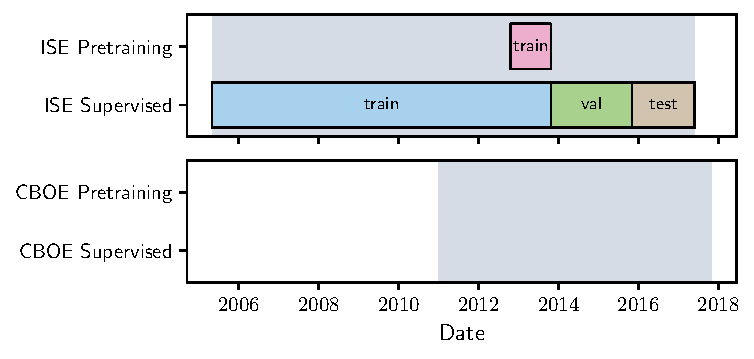
\includegraphics{train-test-split.pdf}
    \caption[Training Scheme on \glsentryshort{ISE} and \glsentryshort{CBOE} Sample]{Training scheme on \gls{ISE} and \gls{CBOE} sample. The train and validation set are split by time. Shaded area \mysquare{viz-gray} indicates the duration for which the dataset is available.}
    \label{fig:train-test-split}
\end{figure}

Overall, we use \gls{ISE} data from 2 May 2005 to 24 October 2013 to train and data between 25 October 2013 and 5 November 2015 to validate our models. The most recent trades until 31 May 2017 are used to assess the generalization error.

Models are pre-trained on unlabeled samples from the last six months of the training period. Given the significantly larger number of unlabeled customer trades, the pre-training period is reduced to facilitate training on the available computing resources.

We use the \gls{CBOE} sample past 5 November 2015 as a second test set, as visualized in \cref{fig:train-test-split}. Our evaluation approach is the most rigorous as it disallows any form of adaptation of the models, thereby ensuring a rigorous evaluation. Unlike transfer learning techniques such as parameter or model transfer, which expectedly improve model performance, we choose to forgo these techniques and demonstrate the effectiveness of our models without any transfer of knowledge. The start date ensures that leakage from the \gls{ISE} set is minimized.\footnote{The datasets contain features, such as the \gls{NBBO}, that are identical for both sets, assuming trades were executed at both exchanges simultaneously. Also, quotes can be identical between exchanges, if market makers quote at the \gls{NBBO}, which is common practice as documented in \textcite[][10]{securitiesandexchangecommissionReportConcerningExaminations2007}. Utilizing the full \gls{CBOE} sample could result in exaggerated performance estimates if the corresponding \gls{ISE} trade is used in training.}

Our train-test-split assumes that all subsets are drawn from the same distribution, so fitting a classifier on the training set and optimizing for the validation set provides good estimates for the test set. To validate this assumption, we use adversarial validation. Specifically, we re-label all training samples with $y=-1$ and all trades of the validation set with $y=1$, train a classifier on a random subset of the composed dataset, and predict class conformance. The performance is estimated using the \gls{MCC} of \textcite[][445]{matthewsComparisonPredictedObserved1975}, which ranges between $\left[-1, 1\right]$ and is insensitive to class imbalances.\footnote{Classes are imbalanced, due to the training set being $3\times$ the size of the validation set.} Assuming train and validation samples are sampled from the same distribution, the performance estimate is near a random guess, or $\operatorname{MCC} = 0$. For the mid-sized feature set, the \gls{MCC} is \num{0.364260805498287} suggesting training and validation sets are approximately similar. The next section discusses techniques used in training the classifiers.

\subsection{Training and Tuning}\label{sec:training-and-tuning}

The following section describes the experimental setup. For reproducibility, the implementation and experiment tracking are publicly available.\footnote{Code is available at~\url{https://github.com/KarelZe/thesis}. Experiments are tracked at \url{https://wandb.ai/fbv/thesis}.}

\subsubsection{Training of Supervised
    Models}\label{sec:training-of-supervised-models}

Our implementation of \glspl{GBRT} is based on CatBoost \autocite[][5--6]{prokhorenkovaCatBoostUnbiasedBoosting2018} because of its efficient implementation on \glspl{GPU} and native support for categorical variables. 

\begin{figure}[H]
    \centering
    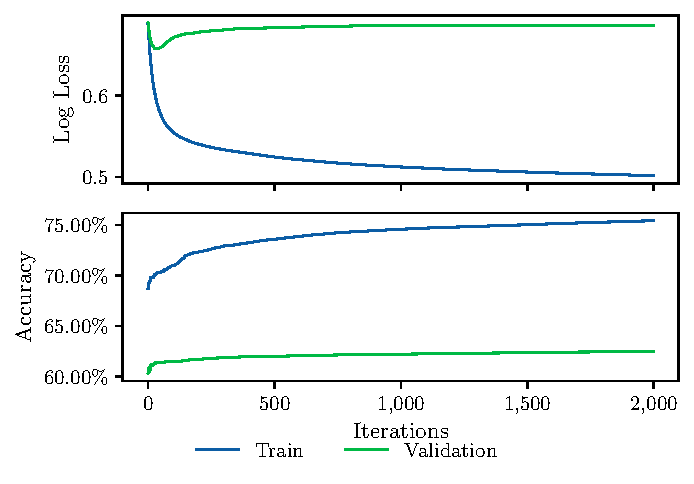
\includegraphics{gbm-train-val-loss-acc.pdf}
    \caption[Training and Validation Accuracy of Gradient Boosting]{Training and validation accuracy of \gls{GBRT} on \gls{ISE} sample. Metrics are estimated on the feature set classic. One iteration corresponds to an additional regression tree added to the ensemble.}
    \label{fig:gbm-train-val-loss-acc}
\end{figure}

\cref{fig:gbm-train-val-loss-acc} displays the loss and accuracies of the default implementation on the \gls{ISE} training and validation set using classical features. The plots reveal several insights. First, the model overfits the training data, as evident from the generalization gap between training and validation accuracies. To improve generalization performance, we apply regularization techniques. Second, validation loss spikes for larger ensembles, while validation accuracy continues to improve. This discrepancy suggests that the predicted class's correctness improves, but the ensemble becomes less confident in the correctness of the prediction.

\begin{figure}[!h]
    \centering
    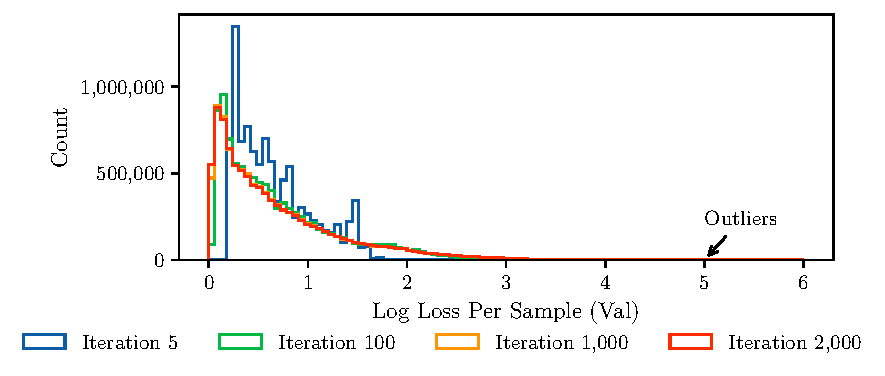
\includegraphics{gbm-loss-distribution.pdf}
    \caption[Sample-Wise Loss of Gradient Boosting]{Sample-wise log loss of \glsentryshort{GBRT} on \glsentryshort{ISE} sample as equi-width histogram. Loss is estimated on the classical feature set. In general, log loss improves for larger ensembles, as indicated by the increased number of samples accumulating around zero but few predictions contribute to the loss unproportionally causing the log loss to stagnate on average.}
    \label{fig:gbm-loss-distribution}
\end{figure}

This behavior can be explained by the log loss being unbound, where single incorrect predictions can cause the loss to explode. We verify this assumption by plotting the distribution of the sample-wise log loss in \cref{fig:gbm-loss-distribution}. As visible, loss per sample decreases for larger ensembles, at the same time few predictions contribute to the loss unproportionally, causing the average validation loss to stagnate.

\begin{figure}[ht]
    \centering
    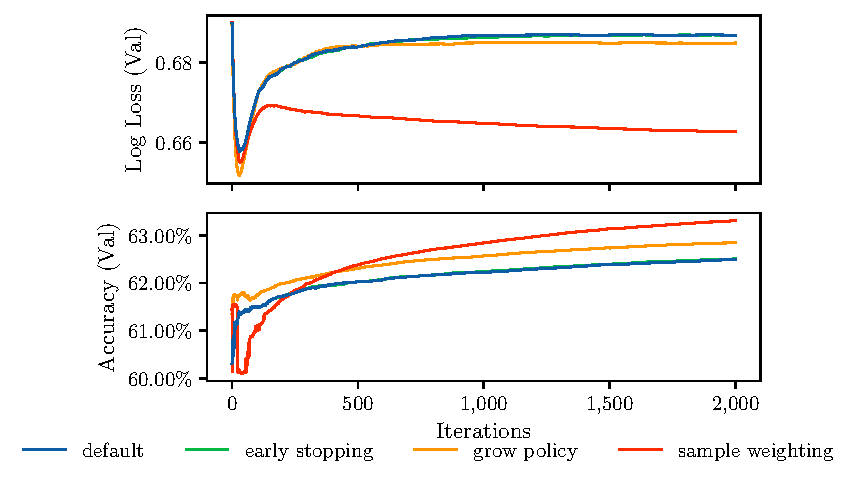
\includegraphics{gbm-optimisations-loss-acc.pdf}
    \caption[Training and Validation Accuracy of Gradient Boosting with Optimisations]{Training and validation accuracy of \gls{GBRT} on \gls{ISE} sample with optimizations. Metrics are estimated on the classical feature set. One iteration corresponds to an additional regression tree added to the ensemble. Loss is expected to decrease for more complex ensembles and accuracy to increase.}
    \label{fig:gbm-optimizations-loss-acc}
\end{figure}

We leverage several architectural changes to reduce the loss, further improve performance and mitigate overfitting in gradient boosting, as shown in \cref{fig:gbm-optimizations-loss-acc}, where the effects on validation accuracy and log loss over the default configuration are visualized. Following standard practice, e.g., \textcite[][]{tuningplaybookgithub}, all other parameters are kept at their default values, while a single parameter is varied to derive the plots. Although this approach ignores parameter interactions, it still can guide the optimal training configuration. We train on the \gls{ISE} training set with classical features and report metrics on the validation set.

\emph{Growth Strategy}

To improve performance, we switch to a leaf-wise growth strategy, following \textcite[][786]{chenXGBoostScalableTree2016}. By default, CatBoost grows oblivious regression trees, which are symmetric and grown level-wise. In this strategy, splits are performed on the same feature and split values across all nodes of a single level, which is computationally efficient but may compromise performance. In contrast, leaf-wise growth selects terminal nodes that provide the largest improvement in the loss, potentially leading to nodes within the same level being split with different features and values, resulting in a closer fit to the data. Leaf-wise growth also aligns with the intuition of split finding from \cref{sec:decision-tree}. This change improves validation accuracy by \SI{0.3461}{\percent} but has little effect on the loss.

\emph{Sample Weighting}

The work of \textcite[][35]{grauerOptionTradeClassification2022} suggests a strong temporal shift in the data, with the performance of classical trade classification rules deteriorating over time.  As a result, the predictability of features derived from these rules diminishes over time, and patterns learned from old observations become less relevant for predicting test samples. To address this, we introduce a sample weighting scheme that assigns higher weights to recent training samples and gradually decays weights over time, which we incorporate into the log loss. Validation and test samples are equally weighted. Sample weighting proves to be essential for achieving high validation performance, and it positively impacts the accuracy and confidence in the prediction mitigating the problem from above.

\emph{Border Count}

In regression trees of gradient boosting, the split finding is typically approximated with quantization, whereby all numeric features are first discretized into a fixed number of buckets through histogram building, and splits are evaluated at the border of the buckets \autocite[][3147]{keLightGBMHighlyEfficient2017}. To increase the number of split candidates, we raise the border count to \num{254}. Generally, this leads to increased accuracy at the cost of computational efficiency. Yet, in the experiment above, the improvements in validation loss and accuracy are minor compared to the previous modifications.

\emph{Early Stopping and Checkpointing}

To reduce overfitting, we monitor the training and validation accuracies when adding new trees to the ensemble and suspend training once validation accuracy decreases for \num{100} iterations. The ensemble is then cut back to achieve the highest validation accuracy. In the experiment above, early stopping does not apply, as validation accuracy continues to improve for larger ensembles. We employ additional measures to address overfitting but treat them as a tunable hyperparameter, with further details provided in \cref{sec:hyperparameter-tuning}. We incorporate all ideas into our large-scale studies.

\textbf{FT-Transformer}

We rely on the FT-Transformer of \textcite[][18935--18936]{gorishniyRevisitingDeepLearning2021} as our second model. The training of Transformers has been found non-trivial and requires a carefully designed training setup of model, optimizer, and learning rate schedule \autocite[][5747]{liuUnderstandingDifficultyTraining2020}. We investigate minor modifications to the default FT-Transformer to stabilize training and improve overall performance. The default FT-Transformer is trained for 10 epochs on the \gls{ISE} dataset with classical features and loss and accuracy are visualized in \cref{fig:fttransformer-optimizations-loss-acc}.\footnote{Default configuration documented in \textcite[][sup.]{gorishniyRevisitingDeepLearning2021}.}

The convergence behavior of our model is similar to that of gradient boosting. Equally, a significant generalization gap exists between the training and validation loss. The training loss decreases sharply, while the validation loss spuriously improves over its initial estimate. Despite this, validation accuracy improves throughout the entire training cycle. We reason that the network learns to correctly classify trades, indicated by the improved accuracy, but only attains low-confident correct predictions or confident but erroneous predictions which both contribute to a large validation loss.

\begin{figure}[!ht]
    \centering
    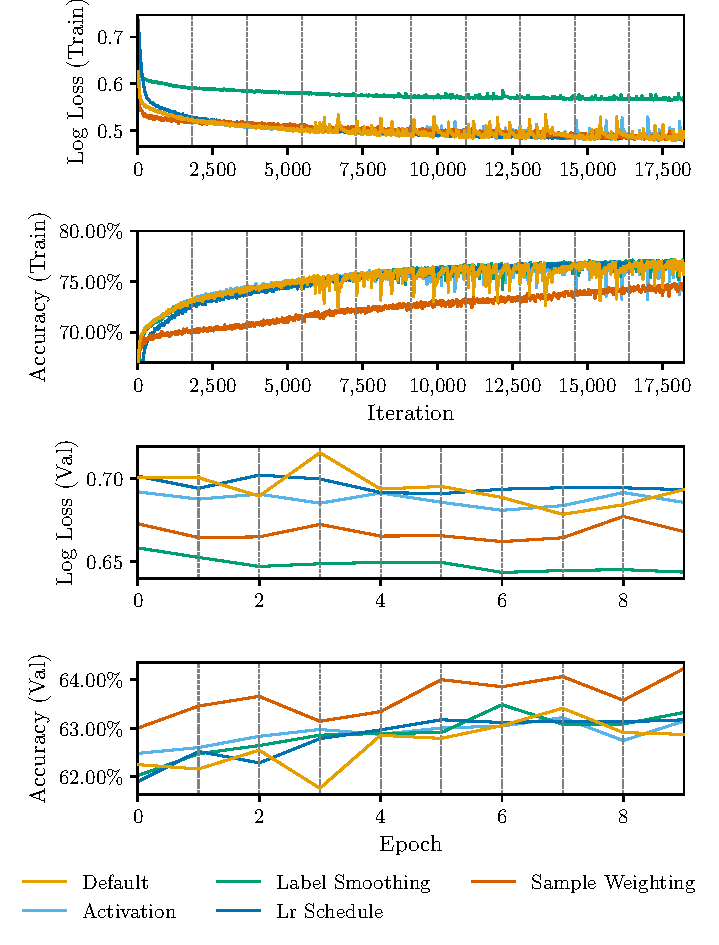
\includegraphics{fttransformer-optimisations-loss-acc.pdf}
    \caption[Training and Validation Accuracy of FT-Transformer with Optimisations]{Training and validation accuracy of FT-Transformer on \gls{ISE} sample with optimizations. Metrics are estimated on the classical feature set. One iteration corresponds to one gradient update. The end of each epoch is marked with a dashed bar. Loss is expected to decrease throughout training and accuracy to increase.}
    \label{fig:fttransformer-optimizations-loss-acc}
\end{figure}

\textbf{Solutions For FT-Transformer}

\emph{Activation Function}

Motivated by previous research, we experiment with replacing the $\operatorname{ReLU}$ activation with the $\operatorname{GELU}$ activation function \autocite[][2]{hendrycksGaussianErrorLinear2020} in the classification head and the gated variant $\operatorname{ReGLU}$ with the gated variant $\operatorname{GEGLU}$ \autocite[][2]{shazeerGLUVariantsImprove2020} in the \gls{FFN}. As visualized in \cref{fig:fttransformer-optimizations-loss-acc}, no advantage in terms of validation accuracy or loss is evident.

\emph{Sample Weighting}

We apply the concept of sample weighting from \gls{GBRT} to Transformers. Specifically, we scale the contribution of individual training samples to the loss using a sample weight, which penalizes the model for misclassifying recent observations. This method is crucial for achieving low validation loss and high validation accuracies, as visible in \cref{fig:fttransformer-optimizations-loss-acc}. The significantly lower training accuracy implies, that patterns from latter observations do not universally transfer to previous observations. It remains unclear what is causing the data drift within the training set.

\clearpage

\emph{Label Smoothing}

A major problem in classification with neural networks is, that the network becomes overconfident in predicting training samples but performs poorly on unseen data. In \cref{fig:fttransformer-optimizations-loss-acc} the effect is evident, as the increased confidence in the prediction on the training set does not transfer to the validation set. To regularize the network, we experiment with label smoothing \autocite[][2823]{szegedyRethinkingInceptionArchitecture2016} by training on soft labels with an uncertainty constant of $\epsilon$. Instead of assigning hard class probabilities of 0 or 1, we assume that true labels in the training set are correct with $1-\epsilon$ probability and incorrect otherwise. For $\epsilon=\num{0.1}$, a trade with the true label $-1$ is assumed to be \SI{90}{\percent} seller-initiated and \SI{10}{\percent} buyer-initiated. While we observe that label smoothing improves the validation loss and reduces the generalization gap, we find that it has a negligible effect on validation accuracy and therefore abandon the approach.

\emph{Learning Rate Schedule}

When training Transformers, the learning rate is often adjusted throughout the training process. \textcite[][6007]{vaswaniAttentionAllYou2017} use a learning rate warm-up period, whereby the learning rate is linearly increased in the early stages of training, followed by decay using an inverse square root learning rate schedule. The warm-up phase is thought to stabilize gradients as weight updates are considerably smaller. According to \cref{sec:residual-connections-layer-norm}, learning rate warm-up is crucial for training post-norm Transformers, but optional for pre-norm Transformers like the FT-Transformer. Nevertheless, we experiment with the effect of learning rate warm-up in our setting and combine a linear warm-up for two epochs with subsequent cosine decay, as visualized in \cref{fig:lr-lin-warmup-cosine-decay}.

\begin{figure}[!ht]
    \centering
    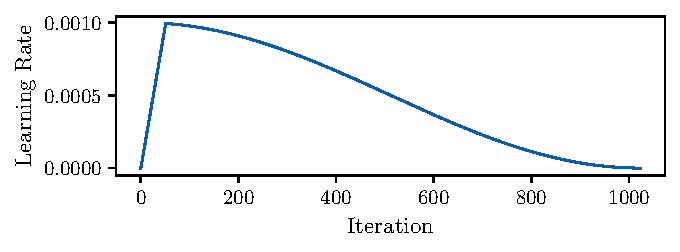
\includegraphics{lr-lin-warmup-cosine-decay.pdf}
    \caption[Linear Learning Rate Warm-Up With Cosine Decay]{Linear learning rate warm-up with cosine decay. Warm-up is performed for the first \SI{5}{\percent} of iterations. In the example, the maximum learning rate is \num{1e-3}.}
    \label{fig:lr-lin-warmup-cosine-decay}
\end{figure}

The scheduled learning rate smooths the training loss and accuracy estimates, as evident in \cref{fig:fttransformer-optimizations-loss-acc}. Therefore, we adopt a training setup with a learning rate schedule, despite the negative effects on training time. The learning rate itself is tuned as part of \cref{sec:hyperparameter-tuning}.

\emph{Batch Size}

% 20 epochs (\num{36460} / \num{145840} iterations) 
We use a fixed batch size of \num{8192} samples for the feature set classic/size and \num{2048} for the feature set option, which is the largest possible size on our \gls{GPU}. Training is performed for \num{20} epochs at maximum. All samples within the training and validation set are shuffled randomly to promote convergence. Although a smaller batch size could enhance the generalization capabilities of the model, as found in \textcite[][3]{keskarLargeBatchTrainingDeep2017}, we train on the largest number of trades per iteration, to optimize throughput. Additional regularization is added to the model, but treated as a tunable hyperparameter.

\emph{Early Stopping and Checkpointing}

Similar to the \gls{GBRT}, we halt training prematurely based on a consecutive decrease in validation accuracy. We set the patience to \num{10} epochs and restore the best model in terms of validation accuracy from the checkpoint. Checkpoints are saved at the end of each epoch. In the experiment above, early stopping does not apply.

\emph{Optimizer}

In line with \textcite[][18937]{gorishniyRevisitingDeepLearning2021}, we train the models using the AdamW optimizer \autocite[][2--3]{loshchilovDecoupledWeightDecay2019} with the standard hyperparameters.\footnote{Parameters $\beta_{1}=0.9, \beta_{2}=0.999$, and $\epsilon = \num{1e-8}$.} The weight decay coefficient in AdamW determining the degree of regularization is tuned in \cref{sec:hyperparameter-tuning}. Weight decay is selectively applied and excludes embeddings, normalization layers, and biases.

In summary, we extend the training setup of \textcite[][18937]{gorishniyRevisitingDeepLearning2021} with a sample weighting scheme and learning rate schedule aimed at boosting performance and training stability.

\vskip 1.3in

\textbf{Solutions For Classical Rules}

Classical trade classification rules serve as a benchmark in our work. We implement them as a classifier that combines arbitrary trade classification rules through stacking, as covered in \cref{sec:semi-supervised-approaches}.

In cases where classification is not feasible due to missing data or the rules' definition itself, we resort to a random classification, which achieves an average accuracy of \SI{50}{\percent}. The approach is adopted from \textcite[][887]{savickasInferringDirectionOption2003}.

\subsubsection{Training of Semi-supervised
    Models}\label{sec:training-of-semi-supervised-models}

This section discusses the extensions necessary to train the semi-supervised variants of \glspl{GBRT} and the FT-Transformer.

\textbf{Gradient Boosting With Self-Training}

To incorporate unlabeled trades into the training procedure, we combine gradient boosting with a self-training classifier, as derived in \cref{sec:extensions-to-gradient-boosted-trees}. We repeat self-training for 2 iterations and require the predicted class probability to exceed $\tau=0.9$. As the entire ensemble is rebuilt three times, the low number of iterations and high confidence threshold, strike a balance between computational requirements and the need for high-quality predictions. The base classifier is otherwise identical to supervised gradient boosting from \cref{sec:training-of-supervised-models}.

\textbf{FT-Transformer With Pre-Training}

The FT-Transformer is trained in two stages. First, we train for \num{20} epochs on unlabeled \gls{ISE} trades using the \gls{RTD} head, followed by \num{20} epochs of fine-tuning on labeled \gls{ISE} training data with the binary classification head.

During pre-training and fine-tuning, early stopping is applied based on the value of the objective on the validation set, using patience of \num{10}. This particular setup is adopted from \textcite[][15]{rubachevRevisitingPretrainingObjectives2022} for being compute-efficient and offering competitive performance on tabular datasets. The hidden dimension of the classification head is set to \num{512}. Based on \textcite[][3]{clarkElectraPretrainingText2020} \SI{15}{\percent} of all tokens are replaced.

Since the unlabeled sample includes various types of trades that may not be comparable to the labeled sample, we update all layers during fine-tuning. Empirically, fine-tuning the entire model is among the most successful methods, as results from \textcite[][104--105]{raeScalingLanguageModels2022} for Transformers in general and results from \textcite[][39]{merchantWhatHappensBERT2020} specific for \gls{BERT}-like architectures document. Yet, updating all layers is the most resource-intensive.

Following \textcite[][4]{rubachevRevisitingPretrainingObjectives2022}, the learning rate and weight decay are shared between the pre-training and fine-tuning stages. All other hyperparameters related to the model are identical.

\subsubsection{Hyperparameter Tuning}\label{sec:hyperparameter-tuning}

All of our machine-learning models feature a set of tunable hyperparameters. The results of previous studies, exemplary the one of \textcite[][511]{grinsztajnWhyTreebasedModels2022}, emphasize the need for tuning routines, as the test performance of the FT-Transformer and \glspl{GBRT} largely fluctuates with the hyperparameter configuration. Classical rules have no hyperparameters per se, but the best hybrid rules can be attained through hyperparameter search.
For a fair comparison, we employ an exhaustive hyperparameter search, to find a suitable hyperparameter configuration for each of our models.

\textbf{Bayesian Search}

We run a novel Bayesian search to suggest and tune the hyperparameters automatically. In Bayesian search, a prior belief for all possible objective functions is formulated from the parameter intervals, which is then gradually refined by updating the Bayesian posterior with data from previous trials thereby approximating the likely objective function \autocite[][149]{shahriariTakingHumanOut2016}. Compared to brute-force approaches, such as grid search, unpromising search regions are omitted, resulting in more promising trials.

While different algorithmic implementations exist for Bayesian optimization, we choose the \emph{Optuna} library \autocite[][2623--2631]{akibaOptunaNextgenerationHyperparameter2019}, which implements the tree parzen estimator algorithm and is capable of handling both continuous and categorical hyperparameters.\footnote{Implementation of the tree-parzen estimator searches the first 10 trials randomly before the completed trials affect the sampling.} We maximize the accuracy of the validation set, which is also our decisive metric for evaluation (cp. \cref{sec:evaluation-metric}), and run $\num{50}$ trials per feature set for the \gls{GBRT} and $\num{10}$ trials for the FT-Transformer. The best combination of each is tested out-of-sample in \cref{sec:results}.

\textbf{Gradient Boosting}

Our search space is reported in \cref{tab:hyperparameter-space-gbm}, which is loosely aligned with \textcites[][sup.]{gorishniyRevisitingDeepLearning2021}[][sup.]{prokhorenkovaCatBoostUnbiasedBoosting2018}.

\begin{table}[!ht]
    \centering
    \sisetup{table-number-alignment=left}
    \caption[Hyperparameter Search Space of Gradient Boosting]{Hyperparameter search space of gradient boosting.}
    \label{tab:hyperparameter-space-gbm}
    \begin{tabular}{@{}ll@{}}
        \toprule
        Hyperparameter               & Distribution                                  \\ \midrule
        Depth                        & $\operatorname{UniformInt}[1,12]$             \\
        Learning rate $\eta$         & $\operatorname{LogUniform}[0.001, 0.125]$     \\
        $\ell_2$ Leaf regularization & $\operatorname{UniformInt}[2, 30]$            \\
        Random strength              & $\operatorname{LogUniform}[\num{1e-9}, 10.0]$ \\
        Bagging temperature          & $\operatorname{Uniform}[0.0, 1.0]$            \\ \bottomrule
    \end{tabular}
\end{table}

As documented, we tune five hyperparameters for gradient boosting. The first is the depth, which determines the number of levels in each tree. Other than \textcite[][sup.]{gorishniyRevisitingDeepLearning2021}, we increase the upper bound to twelve to allow for more complex ensemble members. Acknowledging the research of \textcite[][1203]{friedmanGreedyFunctionApproximation2001} that the learning rate \eta~and the size of the ensemble have a strong interdependence, we only tune the learning rate and stop extending the ensemble based on the early stopping criterion. Random strength, bagging temperature, and $\ell_2$ leaf regularization are measures to counter overfitting. Specifically, random strength controls the degree of Gaussian noise added to the scores of split candidates to introduce randomness in the selected splits. In a similar vein, the algorithm introduces randomness on the sample level through Bayesian bootstrap \autocite[][130--131]{rubinBayesianBootstrap1981}. The hyperparameter controls the distribution used for sampling, and implicitly the aggressiveness of bagging. Finally, $\ell_2$ leaf regularization adds a penalty term to the terminal leaf's estimates. The hyperparameter controls the degree of regularization.

\begin{figure}[!ht]
    \subfloat[Hyperparameter Search Space of \gls{GBRT} With Feature Set Classic\label{fig:ise-gbm-hyperparam-classical}]{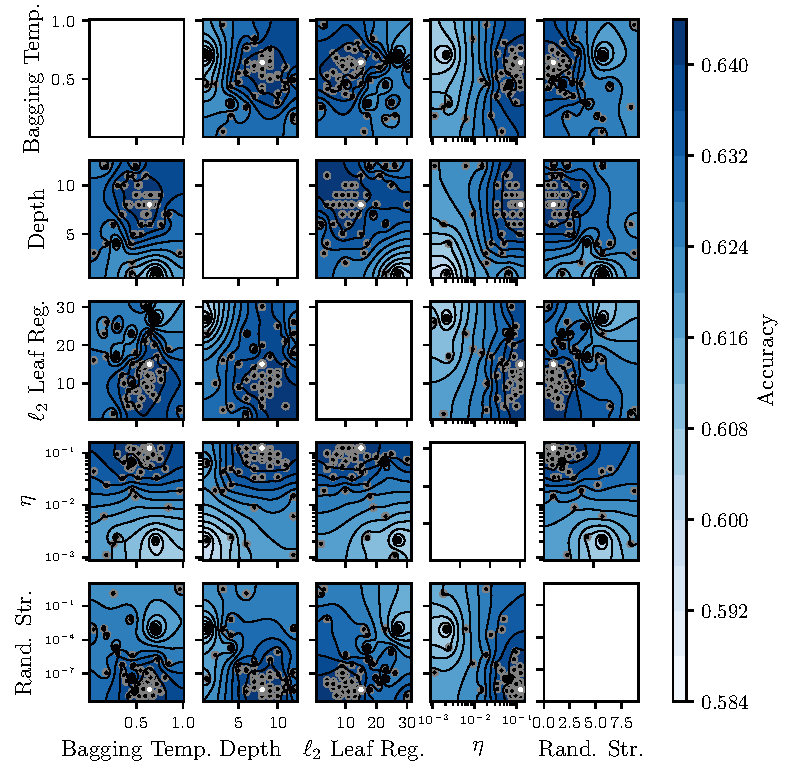
\includegraphics[width=0.6\textwidth]{1gzk7msy-hyperparam-search-space.pdf}}
    \vfill
    \subfloat[Hyperparameter Search Space of \gls{GBRT} With Feature Set Size\label{fig:ise-gbm-hyperparam-classical-size}]{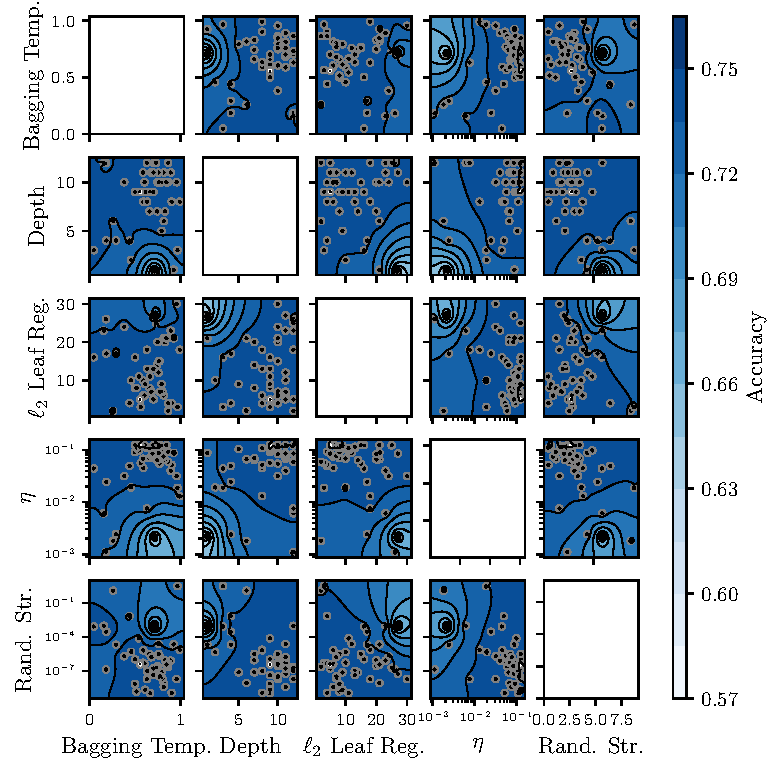
\includegraphics[width=0.6\textwidth]{3vntumoi-hyperparam-search-space.pdf}}
    \caption[Hyperparameter Search Space of Gradient Boosting]{Hyperparameter Search Space of \gls{GBRT} on \gls{ISE} Validation Set}
    \label{fig:ise-gbm-hyperparam}
\end{figure}
\clearpage
\begin{figure}[!ht]
    \ContinuedFloat
    \subfloat[Hyperparameter Search Space of \gls{GBRT} With Feature Set Option\label{fig:ise-gbm-hyperparam-ml}]{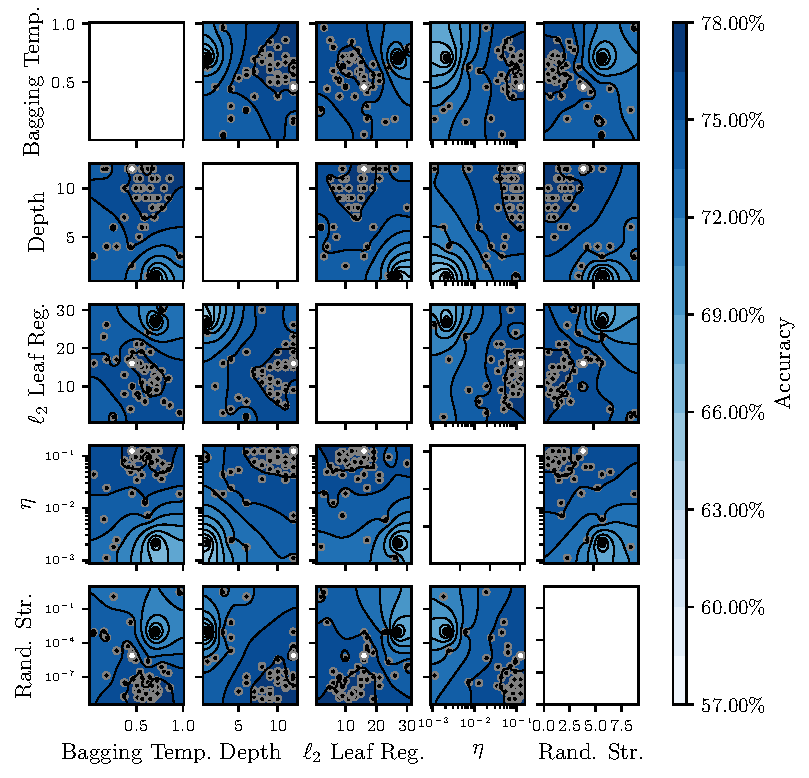
\includegraphics[width=0.6\textwidth]{2t5zo50f-hyperparam-search-space.pdf}}
\end{figure}

\cref{fig:ise-gbm-hyperparam-classical} visualizes the hyperparameter search space of the \gls{GBRT} on the \gls{ISE} dataset with classical features, from which we can derive several observations. First, hyperparameter tuning has a significant impact on the prediction, as the validation accuracy varies between \SI{58.429}{\percent} and \SI{64.378}{\percent} for different trials. Second, the best hyperparameter combination, marked with \bestcircle, lies off-the-borders surrounded by other promising trials, indicated by the contours, from which we can conclude, that the found solution is a stable and reasonable choice for further analysis.

In \cref{fig:ise-gbm-hyperparam-classical-size} we repeat the analysis for \glspl{GBRT} trained on size features. The loss surface is smooth with large connected regions. As the best solution achieving \SI{75.03504680858162}{\percent} accuracy lies within a splayed region of dense sampling, it is a good choice for further analysis. Consistent with the loss surface of \cref{fig:ise-gbm-hyperparam-classical}, the trees are grown to the maximum depth and a high learning rate, indicating the need for complex ensemble members highly corrective to previous predictions. Part of this could be due to the low signal-to-noise ratio in financial data.

The loss surface of the \gls{GBRT} trained on the feature set including option features is the least fragmented. While the validation accuracy of the best combinations improves significantly to \SI{76.99459643967347}{\percent}, worst trials even underperform these of smaller feature sets. We note, more data does not per se improve the model and that models require a thoughtful tuning procedure. Our conclusion contradicts the one of \textcite[][14]{ronenMachineLearningTrade2022}, who find no advantage in tuning tree-based ensembles for trade classification. Results are tabulated in \cref{tab:solutions-gbm}.

\begin{table}[!ht]
    \centering
    \sisetup{table-format=3.2,table-alignment-mode = none, table-number-alignment=left, table-text-alignment = left}
    \caption[Search Solutions of Gradient Boosting]{Search solutions of gradient boosting. The three right columns document the best combination in terms of validation accuracy per feature set. We perform \num{50} trials.}
    \label{tab:solutions-gbm}
    \begin{tabular}{@{}llSSS@{}}
        \toprule
        Hyperparameter               & Distribution                                  & {\glsentryshort{FS} Classic} & {\glsentryshort{FS} Size} & {\glsentryshort{FS} Option} \\ \midrule
        Depth                        & $\operatorname{UniformInt}[1,12]$             & 8                            & 9                         & 12                          \\
        Learning rate $\eta$         & $\operatorname{LogUniform}[0.001, 0.125]$     & 0.12484221864046671          & 0.12347889459796775       & 0.12471458170177774         \\
        $\ell_2$ Leaf regularization & $\operatorname{UniformInt}[2, 30]$            & 15                           & 5                         & 16                          \\
        Random strength              & $\operatorname{LogUniform}[\num{1e-9}, 10.0]$ & \num{4e-9}                   & \num{4e-7}                & \num{8e-6}                  \\
        Bagging temperature          & $\operatorname{Uniform}[0.0, 1.0]$            & 0.6419530220498153           & 0.5574912093427532        & 0.45578836944233            \\ \midrule
        Validation Accuracy in \%    &                                               & 64.37816236230594            & 75.03504680858162         & 76.99459643967347           \\ \bottomrule
    \end{tabular}
\end{table}

\textbf{Gradient Boosting With Self-Training}

The search space for the semi-supervised variant is identical to the supervised gradient boosting. To conserve space, we only report the tabulated results in \cref{tab:solutions-GBRT-self-training}.\footnote{Visualizations of the hyperparameter search space are available online. See \url{https://wandb.ai/fbv/thesis/runs/37lymmzc} for \gls{FS} classic, \url{https://wandb.ai/fbv/thesis/runs/324v3uv5} for \gls{FS} size, and \url{https://wandb.ai/fbv/thesis/runs/t55nd8r0} for \gls{FS} option.}

\begin{table}[!ht]
    \centering
    \sisetup{table-format=3.2,table-alignment-mode = none, table-number-alignment=left, table-text-alignment = left}
    \caption[Search Solutions of Gradient Boosting With Self-Training]{Search solutions of gradient boosting with self-training. The three right columns document the best combination in terms of validation accuracy per feature set. We perform \num{50} trials. Arrows indicate the change compared to the supervised variant.}
    \label{tab:solutions-GBRT-self-training}
    \begin{tabular}{@{}llSSS@{}}
        \toprule
        Hyperparameter               & Distribution                                  & {\glsentryshort{FS} Classic}                                & {\glsentryshort{FS} Size}                                   & {\glsentryshort{FS} Option}                                 \\ \midrule
        Depth                        & $\operatorname{UniformInt}[1,12]$             & 9                                                           & 10                                                          & 9                                                           \\
        Learning rate $\eta$         & $\operatorname{LogUniform}[0.001, 0.125]$     & 0.12337960608926582                                         & 0.1248422186404667                                          & 0.12347504812996231                                         \\
        $\ell_2$ Leaf regularization & $\operatorname{UniformInt}[2, 30]$            & 12                                                          & 9                                                           & 13                                                          \\
        Random strength              & $\operatorname{LogUniform}[\num{1e-9}, 10.0]$ & \num{2e-8}                                                  & \num{5e-8}                                                  & \num{5e-8}                                                  \\
        Bagging temperature          & $\operatorname{Uniform}[0.0, 1.0]$            & 0.34010535578784745                                         & 0.5214954412829511                                          & 0.4666577105566224                                          \\ \midrule
        Validation Accuracy in \%    &                                               & {$\textcolor{viz-red}{\downarrow} \num{64.29671279599335}$} & {$\textcolor{viz-red}{\downarrow} \num{74.83010065958079}$} & {$\textcolor{viz-red}{\downarrow} \num{76.41433947686962}$} \\ \bottomrule
    \end{tabular}
\end{table}

Matching the supervised results, semi-supervised ensembles exhaust the maximum tree depth and combine trees with a coarse learning rate. By parameter importance, both are most influential on the final result. Again, this is an indication that the trade data is not easily separable, requiring multiple features and splits. The found hyperparameters for $\ell_2$ leaf regularization, random strength, and bagging are balanced. Overall, the best validation accuracies are slightly inferior to the supervised variant.


\textbf{FT-Transformer}

The search space for the FT-Transformer is identical to \textcite[][sup.]{gorishniyRevisitingDeepLearning2021} (variant (b)) with minor deviations and reported in \cref{tab:hyperparameter-space-2}.

\begin{table}[!ht]
    \centering
    \sisetup{table-format=3.2,table-alignment-mode = none, table-number-alignment=left, table-text-alignment = left}
    \caption[Hyperparameter Search Space of FT-Transformer]{Hyperparameter search space of FT-Transformer.}
    \label{tab:hyperparameter-space-2}
    \begin{tabular}{@{}ll@{}}
        \toprule
        Hyperparameter         & Distribution                                        \\ \midrule
        Layers $L$             & $\operatorname{UniformInt}[1,6]$                    \\
        Attention dropout      & $\operatorname{Uniform}[0, 0.5]$                    \\
        \gls{FFN} dropout      & $\operatorname{Uniform}[0, 0.5]$                    \\
        Weight decay $\lambda$ & $\operatorname{LogUniform}[\num{3e-5}, \num{3e-4}]$ \\
        Learning rate $\eta$   & $\operatorname{LogUniform}[\num{1e-6}, \num{1e-3}]$ \\ \bottomrule
    \end{tabular}
\end{table}

We vary the layer count and the embedding dimension, which directly affect the capacity of the network. Layers refer to the number of Transformer blocks in the encoder stack. The dimension of numerical and continuous embeddings $d_e$ is at \num{256} at maximum, which is half the dimension used in the author's work. We make this sacrifice, due to being computation-bound by the size of the dataset. Dropout in the attention module and the \gls{FFN} is used to prevent overfitting the training data. As discussed in \cref{sec:training-of-supervised-models}, we treat the weight decay term in the weight update rule of the AdamW optimizer as a hyperparameter, with larger values for \lambda~enforcing a stronger shrinkage of weights and thereby reducing overfitting.

Due to the pseudo-random sampling during the first trials of Bayesian search combined with the reduced number of trials for the Transformer studies, the tested hyperparameter combinations are identical for all feature sets, as visible in \cref{fig:ise-transformer-hyperparam}.

\begin{figure}[!ht]
    \subfloat[Hyperparameter Search Space of FT-Transformer With Feature Set Classic\label{fig:ise-transformer-hyperparam-classical}]{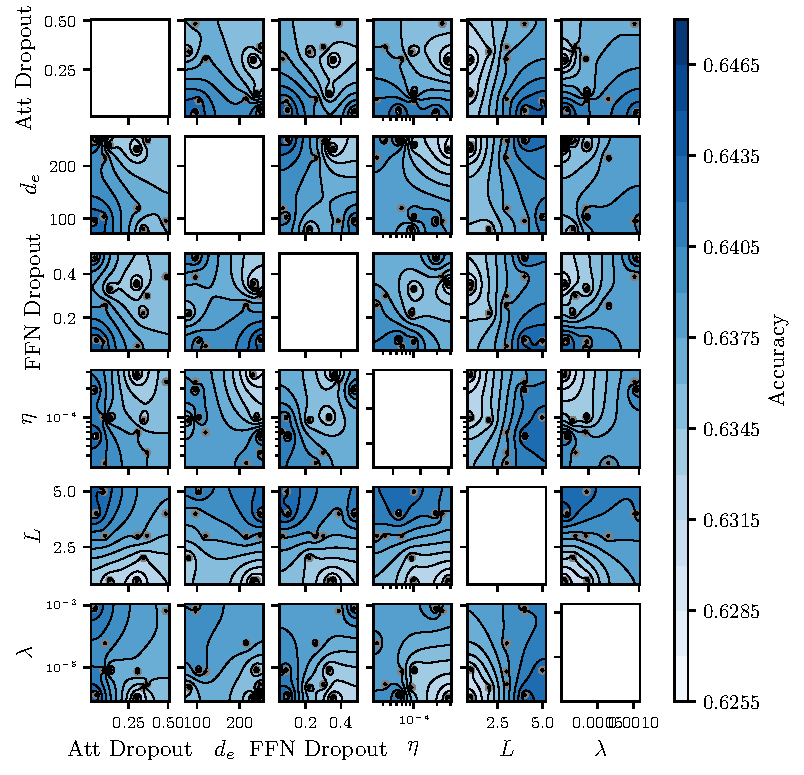
\includegraphics[width=0.6\linewidth]{3jpe46s1-hyperparam-search-space.pdf}}
    \vfill
    \subfloat[Hyperparameter Search Space of FT-Transformer With Feature Set Size\label{fig:ise-transformer-hyperparam-classical-size}]{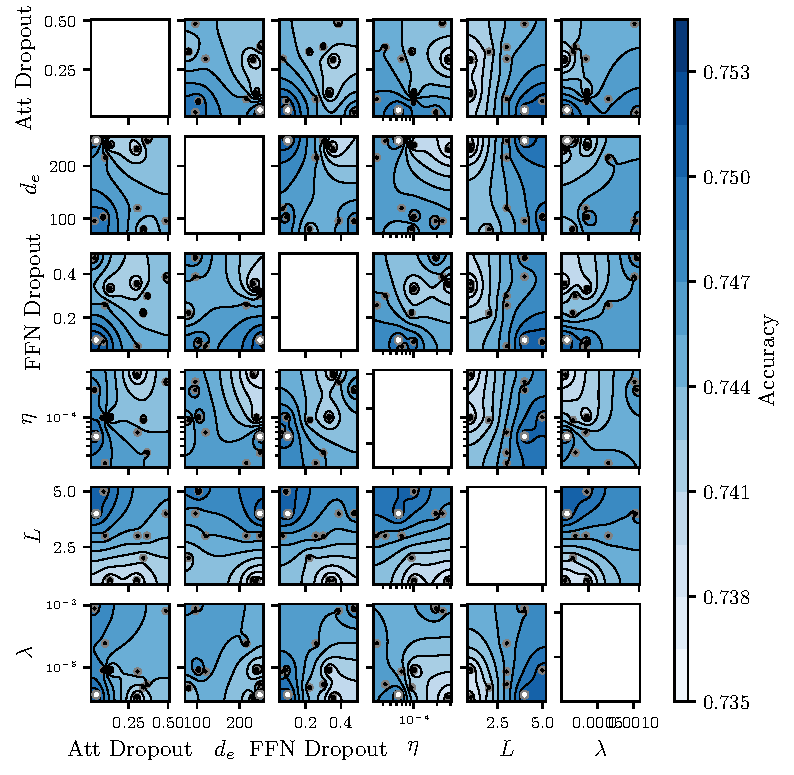
\includegraphics[width=0.6\linewidth]{1qx3ul4j-hyperparam-search-space.pdf}}
    \caption[Hyperparameter Search Space of FT-Transformer]{Hyperparameter Search Space of FT-Transformer on \gls{ISE} Validation Set}
    \label{fig:ise-transformer-hyperparam}
\end{figure}
\clearpage
\begin{figure}[!ht]
    \ContinuedFloat
    \subfloat[Hyperparameter Search Space of \gls{GBRT} With Feature Set Option\label{fig:ise-transformer-hyperparam-ml}]{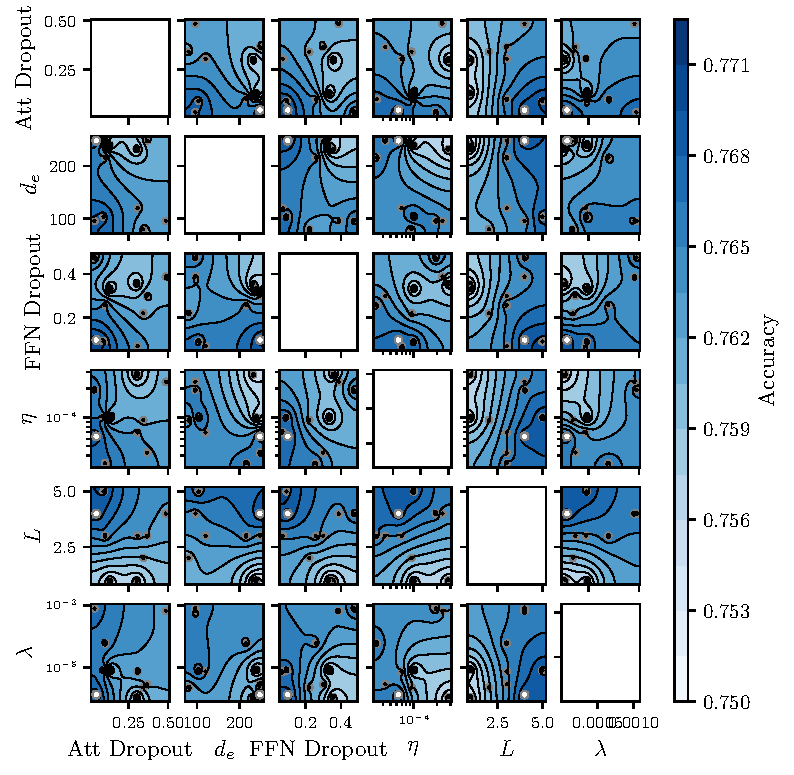
\includegraphics[width=0.6\linewidth]{2h81aiow-hyperparam-search-space.pdf}}
\end{figure}

With the smaller number of trials, the search space is less densely populated. Despite the decreased coverage, for the searched combinations the impact of hyperparameter tuning is less pronounced than for the \gls{GBRT}. As such, accuracies for \cref{fig:ise-transformer-hyperparam-classical} fluctuate between \SI{62.55}{\percent} and \SI{64.65}{\percent}. This translates to other feature sets. Unaffected, the validation accuracies are higher than for gradient boosting.

The best combination is identical for all feature sets. The embedding dimension is at \num{248}, which is almost maxed out and the model uses four Transformer blocks. Thus, it has a medium capacity with \num{1985649} to \num{4252369} parameters, depending on the feature set. From all hyperparameters, the number of layers is most impactful on the final accuracy. While the use of dropout and weight decay for regularization is minimal and marginally affects the validation performance. The large token dimensionality and mid-layer count could be an indication, that few attention heads are enough to extract patterns, but the learned patterns are relatively complex. The search results are compiled in \cref{tab:solutions-transformer}.

\begin{table}[!ht]
    \centering
    \sisetup{table-format=3.2,table-alignment-mode = none, table-number-alignment=left, table-text-alignment = left}
    \caption[Search Solutions of FT-Transformer]{Search solutions of FT-Transformer. The three right columns document the best combination in terms of validation accuracy per feature set. We perform \num{10} trials. A discussion of these results is provided below.}
    \label{tab:solutions-transformer}
    \begin{tabular}{@{}llSSS@{}}
        \toprule
        Hyperparameter                       & Distribution                                        & {\glsentryshort{FS} Classic} & {\glsentryshort{FS} Size} & {\glsentryshort{FS} Option} \\ \midrule
        Layers $L$                           & $\operatorname{UniformInt}[1,6]$                    & 4                            & 4                         & 4                           \\
        Embedding dimension $d_{\mathrm{e}}$ & $\operatorname{UniformInt}[64, 256]$                & 248                          & 248                       & 248                         \\
        Attention dropout                    & $\operatorname{Uniform}[0, 0.5]$                    & 0.04424625102595975          & 0.04424625102595975       & 0.04424625102595975         \\
        \gls{FFN} dropout                    & $\operatorname{Uniform}[0, 0.5]$                    & 0.0979914312095726           & 0.0979914312095726        & 0.0979914312095726          \\
        Weight decay $\lambda$               & $\operatorname{LogUniform}[\num{3e-5}, \num{3e-4}]$ & \num{1e-6}                   & \num{1e-6}                & \num{1e-6}                  \\
        Learning rate $\eta$                 & $\operatorname{LogUniform}[\num{1e-6}, \num{1e-3}]$ & \num{6e-5}                   & \num{6e-5}                & \num{6e-5}                  \\ \midrule
        Validation Accuracy in \%            &                                                     & 64.69                        & 75.42                     & 77.17                       \\ \bottomrule
    \end{tabular}
\end{table}

\vskip 1.3in

\textbf{FT-Transformer With Pre-Training}

The hyperparameter search space for Transformers with a pre-training objective is identical to that shown in \cref{tab:hyperparameter-space-2}. As evident from \cref{tab:solutions-transformer-pretraining}, the found solutions are identical to these of the FT-Transformer without pre-training and identical for all three feature sets. During pre-training, we can detect if a token is replaced with \SI{94.06319856643677}{\percent} to \SI{95.89540958404541}{\percent} accuracy.\footnote{Na\"ive prediction yields \SI{85}{\percent} accuracy given the chosen replacement rate.}

\begin{figure}[!ht]
    \centering
    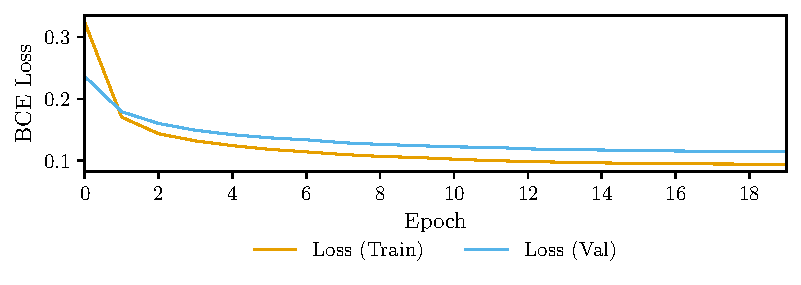
\includegraphics{transformer_ise_pretrain_classical.pdf}
    \caption[Pre-Training Loss of FT-Transformer]{Pre-training loss on \gls{ISE} sample with \gls{FS} classic. Training is performed for 20 epochs. Loss is the mean over all batches per epoch.}
    \label{fig:fttransformer-pretrain-loss}
\end{figure}

Pre-training performance is however bound by the available computing budget. As evident from \cref{fig:fttransformer-pretrain-loss}, the models have not fully converged until the end of pre-training, as the loss on the train- and validation set steadily improves.

Validation accuracy after fine-tuning improves for all models over Transformers without pre-training. As the search space is identically sampled for both variants we can directly attribute the improvements of \SI{0.28}{\percent} to \SI{0.72}{\percent} in validation accuracy to pre-training on unlabeled trades.\footnote{Visualizations of the hyperparameter search spaces are available online. See \url{https://wandb.ai/fbv/thesis/runs/12isqh2m} for \gls{FS} classic, for \url{https://wandb.ai/fbv/thesis/runs/2hv1nayy} for \gls{FS} size, and \url{https://wandb.ai/fbv/thesis/runs/3jbqpp4r} for \gls{FS} option for details.}


\begin{table}[!ht]
    \centering
    \sisetup{table-format=3.2,table-alignment-mode = none, table-number-alignment=left, table-text-alignment = left}
    \caption[Search Solutions of FT-Transformer With Pre-Training]{Search solutions of FT-Transformer with pre-training. The three right columns document the best combination in terms of validation accuracy per feature set. We perform \num{10} trials. Arrows indicate the change compared to the supervised variant.}
    \label{tab:solutions-transformer-pretraining}
    \begin{tabular}{@{}llSSS@{}}
        \toprule
        Hyperparameter                       & Distribution                                        & {\glsentryshort{FS} Classic}                               & {\glsentryshort{FS} Size}                                   & {\glsentryshort{FS} Option}                       \\ \midrule
        Layers $L$                           & $\operatorname{UniformInt}[1,6]$                    & 4                                                          & 4                                                           & 4                                                 \\
        Embedding dimension $d_{\mathrm{e}}$ & $\operatorname{UniformInt}[64, 256]$                & 248                                                        & 248                                                         & 248                                               \\
        Attention dropout                    & $\operatorname{Uniform}[0, 0.5]$                    & 0.04424625102595975                                        & 0.04424625102595975                                         & 0.04424625102595975                               \\
        \gls{FFN} dropout                    & $\operatorname{Uniform}[0, 0.5]$                    & 0.0979914312095726                                         & 0.0979914312095726                                          & 0.0979914312095726                                \\
        Learning rate $\eta$                 & $\operatorname{LogUniform}[\num{3e-5}, \num{3e-4}]$ & \num{1e-6}                                                 & \num{1e-6}                                                  & \num{1e-6}                                        \\
        Weight decay $\lambda$               & $\operatorname{LogUniform}[\num{1e-6}, \num{1e-3}]$ & \num{6e-5}                                                 & \num{6e-5}                                                  & \num{6e-5}                                        \\ \midrule
        Validation Accuracy \%               & Pre-Train                                           & {\num{95.89540958404541}}                                  & {\num{95.64009308815002}}                                   & {\num{94.06319856643677}}                         \\
                                             & Fine-Tune                                           & {$\textcolor{viz-green}{\uparrow}\num{65.13623935106421}$} & {$\textcolor{viz-green}{\uparrow} \num{75.69871634547757}$} & {$\textcolor{viz-green}{\uparrow} \num{77.8904}$} \\ \bottomrule
    \end{tabular}
\end{table}

\textbf{Classical Rules}

Akin to selecting the machine learning classifiers, we select our classical baselines on the \gls{ISE} validation set. This prevents \gls{overfitting} the test set and maintains consistency between both paradigms. For the same reason, baselines are kept constant in the transfer setting on the \gls{CBOE} sample.

Optimizing hybrids of trade classification rules through Bayesian search is experimentally feasible by the stacking paradigm of \cref{sec:stacked-rule} and by treating the rules from \cref{sec:rule-based-approaches} as a tunable hyperparameter. After all, we find no outperformance over hybrid rules already reported in the literature, as documented online.\footnote{For the performance of found combinations see \url{https://wandb.ai/fbv/thesis/runs/3f2m9c6i} and \url{https://wandb.ai/fbv/thesis/runs/16d6e4dk} for details. Experiments are run with \num{500} trials. Performance of rules for literature is documented in \cref{tab:ise-classical}.} Our combinations match or trail the accuracies of rules from \textcite[][13--15]{grauerOptionTradeClassification2022} on the \gls{ISE} validation set. Subsequently, we adopt their combinations as our benchmark, considering them to be the most challenging.

From all candidate algorithms, a combination of quote and tick rules, $\operatorname{quote}_{\mathrm{nbbo}} \to \operatorname{quote}_{\mathrm{ex}} \to \operatorname{rtick}_{\mathrm{all}}$, where the quote rule is first applied to the \gls{NBBO} and then to quotes of the \gls{ISE} followed by the reverse tick rule at inter-exchange level, performs best reaching a validation accuracy of \SI{58.76225138074204}{\percent}. For brevity, we refer to this combination as the \gls{GSU} method (small). It can be estimated using features from feature set classic, which qualifies it as a benchmark.

For the second feature set involving size-related rules, we consider rules that involve the trade size or depth rule. Consistent with the recommendation of \textcite[][15]{grauerOptionTradeClassification2022}, a deep stack of the $\operatorname{tsize}_{\mathrm{ex}} \to \operatorname{quote}_{\mathrm{nbbo}} \to \operatorname{quote}_{\mathrm{ex}} \to \operatorname{depth}_{\mathrm{nbbo}} \to \operatorname{depth}_{\mathrm{ex}} \to \operatorname{rtick}_{\mathrm{all}}$ achieves the highest validation accuracy. We refer to this lengthy combination as the \gls{GSU} method (large). Much of the performance gains are owed to the trade size and depth rules, which reduce the dependence on the reverse tick test as a last resort and provide overrides for trades at the quotes, improving validation accuracy to \SI{69.37267458589436}{\percent}. Due to the extended use of the quoted sizes and trade sizes, it is our benchmark for the second feature set.

In the absence of other baselines, we repeatedly compare against the same rule as a baseline for the third feature set, even if it doesn't involve option-specific features.

When comparing the validation accuracies of classical rules and our classifiers, the validation accuracies of classical rules considerably underperform the learned classifier. \cref{sec:results} discusses if the results hold for the test sets. But before, we present the metrics used
for evaluation.

\subsection{Evaluation}\label{sec:evaluation}

Subsequent sub-chapters discuss metrics for evaluation and measures to retrieve feature importance estimates from the estimators.

\subsubsection{Evaluation Metric}\label{sec:evaluation-metric}

Our goal is to maximize the number of trades, where the predicted trade initiator matches the true trade initiator. We assess the quality of our model’s prediction in terms of \emph{accuracy}, which can be stated as:
\begin{equation}
    % \operatorname{accuracy} \colon \mathbb{R}^{N} \times \mathbb{R}^{N} \to  \left[0, 1\right], \quad 
    \operatorname{accuracy}(\mathbf{y}, \widehat{\mathbf{y}}) = 1 - \frac{1}{N}\sum_{i=1}^{N} \operatorname{L}_{\mathrm{0-1}}(\mathbf{y}_i, \widehat{\mathbf{y}}_i),
\end{equation}
where $\operatorname{L}_{\mathrm{0-1}}(\cdot)$ is the 0-1-loss given by:
\begin{equation}
    % \operatorname{L}_{0-1} \colon \mathcal{Y} \times \mathcal{Y} \to \left[0, 1\right], \quad 
    \operatorname{L}_{\mathrm{0-1}}(y, \hat{y}) = \mathbb{I}\left(y\neq \hat{y}\right).
    \label{eq:0-1-loss}
\end{equation}

Intuitively, from the 0-1-loss we obtain the error rate on the dataset, as for every misclassified trade we count a loss of one and normalize by the number of samples $N$, which gives the normalized 0-1-loss. Notably, the loss is the same for false positives and negatives.

Our datasets are approximately balanced and buyer-initiated trades predicted as seller-initiated and vice versa have similar associated costs, which makes accuracy an ideal choice as a performance metric.\footnote{The \gls{ISE} test set consists of \SI{48.5973}{\percent} of buy trades and \SI{46.1278}{\percent} of the \gls{CBOE} test set are buy trades.} We report the accuracy of the test sets.

\subsubsection{Feature Importance
    Measure}\label{sec:feature-importance-measure}

Naturally, we aim to gain insights into the prediction process and identify relevant features, which fall under the umbrella of \emph{interpretability}.
Following, \textcite[][44--45]{liptonMythosModelInterpretability2017} interpretability can be reached through model transparency or post-hoc interpretability methods. Transparent models provide interpretability through a transparent mechanism in the model, whereas post-hoc methods extract information from the already learned model \autocite[][44--45]{liptonMythosModelInterpretability2017}.

Classical trade classification algorithms, as a rule-based classifier, are transparent with an easily understandable decision process and thus provide interpretability \autocite[][91]{barredoarrietaExplainableArtificialIntelligence2020}. Interpretability, however, decreases for deep, stacked combinations involving a large feature count, when interactions between base rules become more complex and the effect of a single feature on the final prediction more challenging to interpret.

The machine learning classifiers, studied in this work, can be deemed a black box model \autocite[][90]{barredoarrietaExplainableArtificialIntelligence2020}. Due to the sheer size of the network or ensemble, interpretability through transparency is impacted. Albeit, the attention mechanism of Transformers provides some interpretability through the attention mechanism, interpretability across all classifiers can only be reached through \emph{model-agnostic, post-hoc interpretability techniques}.

Thereby, our goal is to estimate how much a feature contributes to the performance of the classifier \emph{overall}, which urges for \emph{global feature attribution measures}. The appropriate approach is guided by the properties of the data. Due to the data-generating process with strongly correlated quotes and trade prices at the exchange and nationwide levels, features are strongly dependent. The redundant feature encoding of ratio features exacerbates this effect. Feature independence, however, is the central assumption of most popular feature importance measures, including \gls{SHAP} or random feature permutation \autocite[][2]{aasExplainingIndividualPredictions2021}. A violation of this constraint for two perfectly correlated, predictive features can have the effect that both are deemed unimportant as the feature importance is distributed between features underestimating the true importance of the feature \autocite[][17215]{covertUnderstandingGlobalFeature2020}. For this reason, we estimate feature importances using \gls{SAGE}, which can account for complex interactions between features and yields global importances. 

\textbf{Shapley Additive Global Importance}

\gls{SAGE} is an additive feature importance measure with its foundations in cooperative game theory. As put forth by \textcite[][4770]{lundbergUnifiedApproachInterpreting2017} feature contributions can be estimated through Shapley values \autocite[][310--312]{shapleyValueNpersonGames1953}. Instead of allocating credit in a cooperative game to players, as in the original Shapley formulation, the problem transfers to assign credit across features based on a value function. Intuitionally, for \gls{SAGE}, credit is distributed among features based on the contribution to the model's performance.

Again, $X$ is a random variable describing the input, $Y$ is the response variable, and $F$ is the classifier. In \gls{SAGE} \autocite[][17215--17216]{covertUnderstandingGlobalFeature2020}, Shapley values $\phi_i(v_F)$ are estimated as:
\begin{equation}
    \phi_i(v_F)=\frac{1}{d} \sum_{S \subseteq D \backslash\{i\}}\left(\begin{array}{c}
        d-1 \\
        |S|
        \end{array}\right)^{-1}(v_F(S \cup\{i\})-v_f(S))
        \label{eq:shapley}
\end{equation}
where $D=\left\{1,\ldots,d\right\}$ is a set of feature indices corresponding to the features $x_1,\ldots,x_d$ and $S\subset D$. Intuitionally, \cref{eq:shapley} estimates Shapley values as the weighted average of the incremental change in the value function, $v_F(S)$, before and after the $i$-th feature is added to the feature subsets $S$. Hereby, the first term $\left(\begin{smallmatrix} d-1 \\|S|\end{smallmatrix}\right)^{-1}$ accounts for the possibilities to choose a $|S|$-strong subset from $D \backslash\{i\}$. 

While subsets of features $X_S = \left\{X_i \mid i \in S \right\}$ can be easily constructed, most classifiers, including ours, cannot handle the absence of features as they require fixed-sized inputs during inference. \textcite[][17213]{covertUnderstandingGlobalFeature2020} mitigate the issue, by marginalizing out the missing features $\bar{S}=D\backslash S$ using the conditional distribution $p(X_{\bar{S}} \mid X_S=x_S)$. Following \textcite[][17215--17216]{covertUnderstandingGlobalFeature2020}, the performance of the model for a given subset of features $S$ and loss function $\operatorname{L}(\cdot)$ can now be estimated by
\begin{equation}
v_F(S)=-\mathbb{E}\left[\operatorname{L}\left(\mathbb{E}\left[F(X) \mid X_S\right], Y\right)\right].
\end{equation}
As important features in a subset lead to a reduction in loss or improvement in performance, the negative sign ensures that the value $v_F(S)$ increases. Together with \cref{eq:shapley} the Shapley values can be estimated. Typically, the cross-entropy loss is chosen as the loss function. As classical rules, yield only hard probabilities, we use the zero-one-loss from \cref{eq:0-1-loss} instead.\footnote{We contribute this loss function to the official implementation \url{https://github.com/iancovert/sage/} as part of this thesis.} 

\textbf{Attention Maps}

In addition to \gls{SAGE}, Transformer-based models offer \emph{some} interpretability through their attention mechanism. Consistent with \textcite[][18]{wiegreffeAttentionNotNot2019} we view attention scores as a vehicle to model transparency.

Recall from our discussion on attention in \cref{sec:attention} that the attention matrix stores how much attention a token pays to each of the keys. Thus, feature attributions can be derived from attention by visualizing features, to which the model attends, in an attention map. While attention maps are specific to Transformers or other attention-based architectures, rendering them useless for cross-model comparisons, they give additional insights from different attention layers and attention heads of the model on a per-trade and global basis.

In the tabular domain, various approaches have been investigated in the literature to obtain attention from multiple attention heads and Transformer blocks. \textcite[][18]{somepalliSaintImprovedNeural2021} and \textcite[][8]{borisovDeepNeuralNetworks2022} gather attention maps from the first attention layer only, and \textcite[][8]{borisovDeepNeuralNetworks2022} additionally obtain feature attributions by taking the diagonal of the attention matrix $\mathbf{A}$ or through column-wise summation. In contrast, \textcite[][18941]{gorishniyRevisitingDeepLearning2021} leverage all attention matrices by averaging over multiple Transformer blocks, attention heads, and samples to obtain global feature attributions. Given \cref{sec:architectural-overview,sec:attention}, where we emphasized the unique role of attention heads and lower sub-layers, both approaches may be myopic, as attention heads contribute unequally to the result, or as later attention layers are neglected altogether.

While not explored systematically in the tabular domain yet, the rollout attention method of \textcite[][4192]{abnarQuantifyingAttentionFlow2020} combines raw attention from multiple layers through recursive matrix multiplication with the weight matrices from attention layers below, as shown in this Equation:\footnote{Notation from adapted from \textcite[][786]{cheferTransformerInterpretabilityAttention2021}.}
\begin{equation}
    \begin{aligned}
        \hat{\mathbf{A}}^{(l)}    & =\mathbf{I}+\mathbb{E}_h \mathbf{A}^{(l)}                                              \\
        \operatorname { rollout } & =\hat{\mathbf{A}}^{(1)} \cdot \hat{\mathbf{A}}^{(2)} \ldots\cdot\hat{\mathbf{A}}^{(L)}
    \end{aligned}
    \label{eq:attention-map-rollout}
\end{equation}

In each layer the raw attention scores $\mathbf{A}^{(l)}$ are averaged over $h$ heads, denoted by $\mathbb{E}_h$. The identity matrix $\mathbf{I}$ is added to account for the residual connections. While rollout attention considers all attention layers in the calculation of feature attributions, it does not consider a signal and attributes equal weights to all attention heads \autocite[][786]{cheferTransformerInterpretabilityAttention2021}.

In an attempt to explain the decision-making process of multi-modal Transformers, including self-attention-based Transformers, \textcite[][399]{cheferGenericAttentionmodelExplainability2021} incorporate gradients to weight the head's contribution when averaging over the heads of a layer, as shown in \cref{eq:attention-map-weighted}. Like before, all attention layers are considered.

\begin{equation}
    \begin{aligned}
        \bar{\mathbf{A}}^{(l)}   & =\mathbf{I} + \mathbb{E}_h\left(\left(\nabla \mathbf{A}^{(l)} \odot \mathbf{A}^{(l)}\right)^{+}\right) \\
        \operatorname {wrollout} & =\bar{\mathbf{A}}^{(1)} \cdot \bar{\mathbf{A}}^{(2)} \ldots \cdot \bar{\mathbf{A}}^{(L)}
    \end{aligned}
    \label{eq:attention-map-weighted}
\end{equation}

In this approach, the element-wise product between the gradient of the attention map $\nabla \mathbf{A}^{(l)}=\frac{\partial y_t}{\partial \mathbf{A}}$ for the model's target class $t$ and the attention map $\mathbf{A}^{(l)}$ is calculated to weight the attention head's importance. As introduced in \textcite[][786]{cheferTransformerInterpretabilityAttention2021}, negative contributions are eliminated to focus on the positive relevance, and the results are averaged over the heads dimension. \cref{eq:attention-map-rollout,eq:attention-map-weighted} can be computed with a single forward pass and are computationally efficient.